
\documentclass{article}


%=========================================================================%
%
% Add optional packages. Some are almost essential.
%
%=========================================================================%

\usepackage[natbib=true,citestyle=authoryear,backend=bibtex]{biblatex}
\addbibresource{library.bib}
%\usepackage{natbib}
\usepackage[dvips]{graphicx}
\usepackage{lipsum}
\usepackage{listings}
\usepackage[utf8]{inputenc} % Input encoding and font encoding
%\usepackage[margin = 1in]{geometry} % Margins
\usepackage{setspace} % Setting the spacing between lines
\usepackage{amsthm, amsmath, amsfonts, mathtools, amssymb} % Math packages
\usepackage{sgame, tikz} % Game theory packages
\usetikzlibrary{trees, calc} % For extensive form games
\usepackage{pgfplots}
\usepackage{subfig} % Manipulation and reference of small or sub figures and tables
\usepackage{multirow,array}
%\usepackage[margin = 1in]{geometry} % Margins
\usetikzlibrary{calc}
\usetikzlibrary{matrix}
\usetikzlibrary{positioning}
\usepackage[mathscr]{euscript}
\usepackage{enumitem}
\usetikzlibrary{3d}
\usetikzlibrary{calc,fadings,decorations.pathreplacing}
\usepackage{bm,color}
\usepackage{makecell}
\usepackage{multicol}
\usepackage{float}
\restylefloat{table}
\usepackage{stackengine}
\usepackage{todonotes}
\usepackage{comment}
\usepackage{caption}
\usepackage[capitalize]{cleveref}

\newcommand\Under[2]{\strut%
  \setstackgap{L}{1.1\normalbaselineskip}%
  \setstackgap{S}{2pt}%
  \smash{\stackunder{#1}{#2}}%
}
\def\LA{\rlap{\scalebox{1.2}[1.5]{\kern2pt\raisebox{-.5pt}{$\leftarrow$}}}}
\def\RA{\rlap{\scalebox{1.2}[1.5]{\kern2pt\raisebox{-.5pt}{$\rightarrow$}}}}
\def\UA{\tclap{\scalebox{1.5}[2.2]{$\uparrow$}}}
\def\DA{\bclap{\scalebox{1.5}[2.2]{$\downarrow$}}}
%\renewcommand\arraystretch{1.5}
\renewcommand*{\nameyeardelim}{\addspace} % remove comma in text citations
\usepackage{pgf}
\usetikzlibrary{arrows}

\newcommand\addvmargin[1]{
  \node[fit=(current bounding box),inner ysep=#1,inner xsep=0]{};
}

% Theorems
\newtheorem{theorem}{Theorem}[section]
\newtheorem{corollary}[theorem]{Corollary}
\newtheorem{lemma}[theorem]{Lemma}
\theoremstyle{definition}

\newtheorem{definition}{Definition}[section]
\newtheorem{proposition}[definition]{Proposition}
%\newtheorem{theorem}[definition]{Theorem}
\newtheorem{notation}[definition]{Notation}
%\newtheorem{example}[definition]{Example}
%\newtheorem{corollary}[definition]{Corollary}
%\newtheorem{lemma}[definition]{Lemma}
\newtheorem{primary statistics}[definition]{Primary Statistics}
\newtheorem{auxiliary statistics}[definition]{Auxiliary Statistics}
%\newtheorem{definition}[theorem]{Definition}
%\newtheorem{proposition}[theorem]{Proposition}
%\newtheorem{notation}[theorem]{Notation}
\newtheorem{examplex}[theorem]{Example}
\newenvironment{example}
  {\pushQED{\qed}\renewcommand{\qedsymbol}{$\diamondsuit$}\examplex}
  {\popQED\endexamplex}


% \let\oldendexample\endexample
% \def\endexample{$\diamondsuit$\oldendexample}



%---------------------------%
% Argmax and Argmin
%---------------------------%
\DeclareMathOperator*{\argmax}{arg\,max} % argmax operator
\DeclareMathOperator*{\argmin}{arg\,min} % argmin operator


% Notation



\title{MC-AIXI-CTW Report}
\author{Elliot Catt, Suraj Narayanan, Arie Slobbe}
\begin{document}
\maketitle

\section{Introduction}
We implement and test an approximation of the AIXI model \citep{hutter2005universal}. The AIXI model is a mathematical “solution” to the general reinforcement learning problem. That is, an AIXI agent solves the problem of maximising expected reward in an unknown, stochastic and partially observable environment. Unfortunately, the AIXI model is incomputable. \citep{veness2011monte} present a down-scaled (i.e. computable) version of AIXI which they call Monte Carlo AIXI Context Tree Weighting, or MC-AIXI-CTW. Our work implements the agent design of Veness and colleagues with the aim to reproduce their experimental results on a variety of reinforcement learning domains.

The following subsections briefly introduce the three main components of the MC-AIXI-CTW agent. A complete description of the AIXI agent can be found in \citep{hutter2005universal}. The Monte Carlo component is described in \citep{kocsis2006bandit}, and the Context Tree Weighting method in \citep{willems1995context}.  Section 2 describes a variety of domains on which we tested our agent, section 3 describes our implementation of MC-AIXI-CTW and how to compile and run the code, and section 4 presents our experimental results on a variety of problem domains and compares them with the results originally obtained by \citep{veness2011monte}.

\subsection{The AIXI agent}
AIXI is a Bayesian optimality notion for general reinforcement learning agents. AIXI interacts with an unknown environment in cycles. In each cycle, the agent executes an action and in turn receives an observation and a reward. (when the environment is fully observable at all times, an observation is called a state; see figure). AIXI aims to choose actions that will on average lead to the best possible outcome. More precisely, AIXI maximises the expected sum of rewards over its lifetime.

Each time the agent takes an action, the environment responds by returning an observation reward pair. The agent integrates the new observation-reward information and the next iteration begins with another action by the agent. In principle, the agent has access to its entire history of action-observation-reward cycles, and unlimited time to compute the next best action.  

\begin{figure}
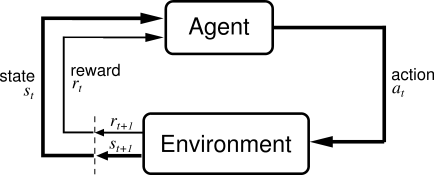
\includegraphics[width = 12cm]{suttonbarto_rl}
	\caption{\citep{sutton1998reinforcement}}
\end{figure}
 

Suppose the AIXI agent interacts with an environment in cycles $k=1,2, \ldots, m$. The agent chooses action $a_k$, subsequently the environment "chooses" (produces) an observation reward pair $o_kr_k$, and the next cycle begins. By interacting, a history sequence $h=a_1o_1r_1 \ldots a_mo_mr_m$ is formed.

Agents are distinguished by how well they choose their actions in light of rewards received from the environment. In cycle $k$, the full AIXI model chooses its next action $a_k$ according to the following equation:

$$a_k \coloneqq \argmax_{a_k} \sum_{o_kr_k} \ldots \max_{a_m} \sum_{o_mr_m} (r_k+\ldots+r_m) \xi (o_1r_1 \ldots o_mr_m \mid a_1 \ldots a_m), $$

where $\xi (o_1r_1 \ldots o_mr_m \mid a_1 \ldots a_m)$ is a mixture environment model over a model class of chronological probability distributions. See \citep{hutter2005universal} for the full details of this model. Intuitively, the agent considers the sum of the total reward over all possible futures up to m steps ahead, weighs each of them by the complexity of programs consistent with the agent’s past that can generate the future, and then picks the action that maximises expected future rewards \citep{veness2011monte}. 

The alternating sum and max operators execute the (finite-horizon) expectimax operation, which is a classic result from sequential decision theory. Expectimax is responsible for planning a best course of action.

The mixture environment model is responsible for learning to predict future observations and rewards based on past experience. The technique is inspired by Solomonoff’s universal induction scheme. Initially, the mixture assigns greater weights to simple environment models. Each interaction cycle generates new evidence as to which models are more likely to be the “true” model of the environment. Models consistent with the evidence acquire increased weight (i.e. importance) in the decision procedure while inconsistent models are pruned away.

The expectimax operation runs in exponential time with respect to lookahead m and is computationally infeasible for all but the smallest values. Worse yet, the mixture environment model is not even finitely computable. To deal with these issues, Veness et al. developed a computable approximation of AIXI. This approximation uses Monte Carlo Tree Search (MCTS) to approximate the expectimax operation and Context Tree Weighting (CTW) to maintain a mixture environment model. 

\subsection{Monte Carlo Tree Search}
Expectimax requires us to consider every possible future that can result from taking an action in the present. Again, this is computationally infeasible. Instead of considering every path through the future, Monte Carlo Tree Search (MCTS) samples as many paths as time and computation resources permit. An action with highly rewarding (simulated) futures is considered better than an action for which every sample returns nothing.

MCTS collects the outcomes of simulations in an iteratively expanding search tree.  \citep{kocsis2006bandit} developed a powerful heuristic which helps the agent focus its resources on useful parts of the tree. Actions with more simulations have better value estimates, so we must carefully consider which actions we care most about investing computational resources in. We prefer to spend resources on actions with high uncertainty about their real value, and/or with high probability of being the best action. These competing demands -- exploration of new actions, and exploitation of known good actions -- are balanced by taking a weighted average in such a way that total “regret” is minimised (see paper).

To illustrate, consider the problem of finding the best opening move in a game of tic-tac-toe. MC-AIXI-CTW runs a number of simulations to up to a pre-specified "search depth" into the future. The Context Tree Weighting method supplies the simulated next board positions (and rewards). In aggregate, the simulations yield an estimated win rate for each opening move. The agent subsequently chooses the opening move that had the highest win rate in its simulations.

\subsection{Context Tree Weighting}
The Context Tree Weighting (CTW) method was initially proposed as a universal compression method. CTW learns to identify patterns in a bit sequence. If the sequence is generated by a D-order Markov process (that is, the probability of the next bit being 1 is conditioned only on the last D bits that were observed) then CTW will converge to optimal prediction. 

Several attributes make CTW a suitable approximator of universal Solomonoff induction:
\begin{itemize}
\item like Solomonoff induction, it maintains a mixture model over environments which converges to the true environment as evidence accumulates;
\item it assigns higher prior probability to simple models;
\item it covers the huge class of D-order Markov processes which contains many interesting and important environments; and
\item its running time is linear in the length of the input sequence, compared to exponential in the length of more na\"ive methods.
\end{itemize}

Each time the agent simulates taking an action, CTW is called to predict the subsequent observation reward pair. In the MC-AIXI-CTW implementation, every action, observation and reward is encoded as a string of bits. So in practice, to generate an observation reward pair, a number of steps are involved. CTW is asked to predict the next bit $b$ given the history sequence $h$, and subsequently we append the predicted bit to the history sequence by setting $h = hb$. We predict subsequent bits in this manner until we have appended to the origininal history $h$ a sequence of bits of length corresponding to an obseration reward pair. 
 
In this manner, the MC-AIXI-CTW agent uses the CTW method to simulate paths through the future in order to plan a best course of action.  By interacting with the environment, MC-AIXI-CTW acquires the training data for CTW to learn over time how to emulate the environment, making it an increasingly good predictor of the future. 

This convergence to the true environment works as follows.
Let $C_D$ denote the class of all prediction suffix trees of depth up to D, which are a form of variable order Markov models. We use $C_D$ as our environment class and we assume that the "true" environment $E^*$ is contained in $C_D$. To each $E \in C_D$ we assign a code with length $CL(E)$. We can think of this code as a compressed representation of the environment; simple environments have simple (short) codes. 

% Explain formula
The mixture environment model $\xi$ from the AIXI model is approximated by 
\begin{equation} \label{eq1}
\begin{split}
\xi (o_1r_1 \ldots o_mr_m \mid a_1 \ldots a_m) &\approx  P_{CTW}(o_1r_1 \ldots o_mr_m \mid a_1 \ldots a_m) \\
 & = \sum_{E \in C_D} P(E) P(o_1r_1 \ldots o_mr_m \mid E, a_1 \ldots a_m) \\ 
 & = \sum_{E \in C_D} 2^{-CL(E)} P(o_1r_1 \ldots o_mr_m \mid E, a_1 \ldots a_m).
\end{split}
\end{equation}

% Explain how convergence to true occurs
The $2^{-CL(E)}$ factor causes simple environments to have an outsize contribution on the output value $P_{CTW}$. The factor $P(o_1r_1 \ldots o_mr_m \mid E, a_1 \ldots a_m)$ approaches zero when the "real" environment $E^*$ produces observation reward pairs $o_1r_1 \ldots o_mr_m$ that we would not likely observe if $E$ were the true environment. Hence, over time the $P(o_1r_1 \ldots o_mr_m \mid E^*, a_1 \ldots a_m)$ term will dominate the sum. 


\section{Overview of implemented domains}
\subsection{Kuhn Poker}
Kuhn Poker is a simplified version of poker from \citep{kuhn1950simplified}. It involves a deck of 3 cards (King, Queen, Jack). First the cards will be given out, and each player bets 1, then the opponent will choose to bet or pass, after looking at his card, the agent will then choose to bet 1 or pass. If the actions taken are equal (both bet or both pass) then the player with the higher card wins the round (King>Queen>Jack). If instead the agent chose to pass, the opponent wins the round. If the opponent passed then the agent bet 1, the opponent then has the choice to bet or pass again, if they pass the agent wins, if they bet 1 then the player with the highest card wins. The opponent will always play the Nash Strategy, to represent this at the start of the round the opponent chooses an $\alpha$ at random between 0 and $\frac{1}{3}$, if they drew a Jack, they will bet with probability $\alpha$, if they drew a queen they will bet with probability 0, if they drew a queen, they will bet 1 with probability $3\alpha$. If they have a second round of betting, they will choose to bet 1 with probability $\alpha+\frac{1}{3}$ regardless of their card. If the agent wins, they get reward equal to the number of chips in play. If the agent loses they will get a reward equal to the negative of the number of chips they bet.


\subsection{Biased Rock Paper Scissors}
Biased Rock Paper Scissors is very similar to regular rock paper scissors, with one exception in how the opponent will choose to play. Both the agent and the opponent will choose either Rock, Paper or Scissors. Rock beats Scissors, Paper beats Rock, Scissors beats Paper. If the agent beats the opponent, the agent will receive a reward of 1, if the agent loses it will receive a reward of 0, if it is a draw, that is both opponent and agent make the same choice, then the agent receives a reward of 0. The opponent repeats its choice of the previous round if it resulted in a win, and picks a move randomly otherwise. 

\subsection{Coin Flip}
The Coin Flip is a very simple environment where the agent will choose heads or tails, a biased coin with probability p for heads and 1-p for tails will be flipped. If the agent guesses correct it will receive reward of 1, if not it will receive a reward of 0.

\subsection{Extended Tiger}
Extended tiger is a simple game where the agent begins sitting on a chair, in front of two doors, behind one door is a tiger, behind the other is some gold. While sitting the agent has the choice to stand or listen to the door, if the agent listens they will observe which door the tiger is behind with a probability of 0.85, and observe the wrong door with probability 0.15. Once standing the agent can open door 1, open door 2. If the agent opens the door with the gold they receive a reward of 30, if they open the door with the tiger they receive a reward of -100. If the agent stands up while sitting down or listens while sitting down they will receive a reward of -1. Any invalid action the agent performs will have a reward of -10.

\subsection{Pacman (POcman, Partially Observable Pacman)}
Partially observable pacman (POcman) is a version of the 17x19 pacman game where the agent controlling Pacman cannot observe the whole space. Instead, pacman can detect if there are walls around him, if he can see a ghost in the four directions around him, if there are is a food pellet within 2, 3, and 4 of his location, if he can see a food pellet in any of the four directions, and if he has the power pill or not. The ghosts will move randomly, unless they are within a manhattan distance of 5 or less in which they will try to move towards him. The agent receives a reward of -1 for every move it makes, -10 for hitting a wall, +10 for collecting a food pellet, -50 touched by a ghost, and +100 if collected all pellets.

\subsection{Tic Tac Toe}
Tic Tac Toe is an adversarial full observable deterministic game played on a 3 by 3 board. It begins with the agent placing a ‘X’ on one of the places on the board, the opponent then places an ‘O’ on another place. This continues until there is a horizontal, vertical or diagonal line of 3 ‘X’s or ‘O’s on the board. At which point the game is over and the player who played the line wins. If the board is full and there is no winner, then the game is a draw. If the agent attempts to place an ‘X’ on a place that already has a piece he will penalized by -3 reward. If the agent loses the game, they get a reward of -2, if the agent wins the game they get a reward of 2, if the agent draws the game it will get a reward of 1. The opponent will always play in a random spot.


\section{Overview of agent program}
TODO: format folder, file, and class names in this section.

The MC-AIXI-CTW agent program is composed of several components. Each is briefly presented in the following overview. More comprehensive documentation is provided in the source files themselves.

The conf folder contains configuration settings for each of the implemented environments, which are kept in the environments folder. 

The AIXI folder holds the Agent class which contains high-level code relating to action selection, model prediction, observation decoding, and action encoding.

The folder named common contains definitions of various functions and constants that are used across the program. 

The file main.cpp reads and parses configuration files, calls various initialisation code, and contains the main agent/environment interaction loop.

The MCTS folder contains the SearchTree and SearchNode classes which implement the UCT algorithm for planning optimal actions within the environment. Veness et al. reconstruct a search tree from scratch at every new cycle. In contrast, our method employs a prune method to reuse as many computations as possible from the previous cycle.

The CTW folder contains the CTNode and ContextTree classes which implement the CTW method for predicting and simulating the environment.


\subsection{Software Architecture}
  \begin{figure}[h]
  \centering
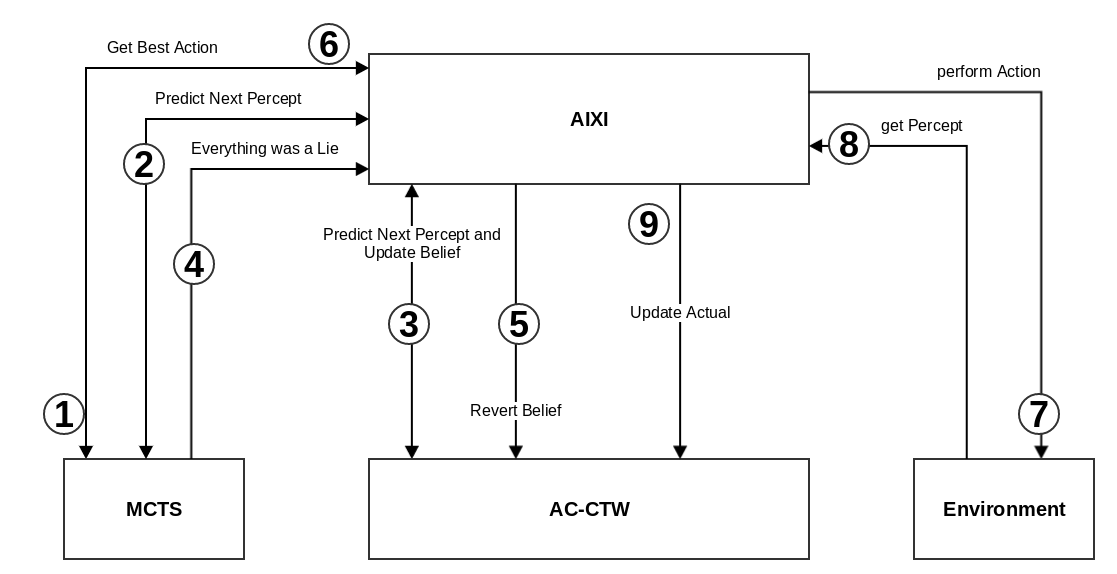
\includegraphics[height=5.5cm]{soft_arch_crop}
\end{figure}

\todo{Add some more explanation}

\subsection{How to compile and run}
\subsubsection*{Linux}
TODO: format terminal commands 
Extract the source files into a folder 
\begin{lstlisting}[language=bash]
~/mc-aixi-ctw 
\end{lstlisting}
 and execute in the terminal:
 
\begin{lstlisting}[language=bash]
cd ~/mc-aixi-ctw
make all
./bin/aixi ./conf/coinflip.conf
\end{lstlisting}

\subsubsection*{Windows (Cygwin)}
\begin{lstlisting}[language=bash]
cd mc-aixi-ctw
make all
/bin/aixi.exe /conf/coinflip.conf
\end{lstlisting}


\subsubsection*{Mac OS}
Extract the source files into a folder ~/mc-aixi-ctw and execute in the terminal:
\begin{lstlisting}[language=bash]
cd ~/mc-aixi-ctw
make all
./bin/aixi ./conf/coinflip.conf
\end{lstlisting}

The file coinflip.conf may be replaced with any other file in the conf folder.
After execution, the two files logfile.log and logfile.csv will contain data on the agent’s actions and performance.




\section{Experimental Results}

Our experimental results for the environments are as follows, we use the following notation,

 \begin{align*}
     D &= \text{ CTW Depth} \\
     m &= \text{ Horizon} \\
     \epsilon &= \text{ Exploration} \\
     \gamma &= \text{ Exploration Decay} \\
     \text{Cycles } &= \text{ Number of cycles } \times 10^3 \\
 \end{align*}
 
Our objective is to test the agent's learning capability in an environment with no prior knowledge. The learnt policy is evaluated at the end of the training phase. For the environments, some are easy such as Biased Rock-Paper-Scissors, and Kuhn-Poker. The other environments TicTacToe, Pacman, Extended Tiger are harder games to learn.




\newpage

\subsection{Biased Rock Paper Scissors}
\begin{tabular}{lllllll}
\centering
Environment & D & m & $\epsilon$ & $\gamma$ & Cycles & Average Reward \\
BRPS        & 32        & 4           & 0.999       & 0.9995            & 30     & 0.2293375        \\
BRPS        & 96        & 8           & 0.999       & 0.9991            & 12     & 0.2419375       \\
BRPS        & 256       & 4           & 0.999       & 0.9991            & 13     & 0.21425        \\
BRPS        & 256       & 8           & 0.999       & 0.999             & 7      & 0.246525        
\end{tabular}

\begin{figure}[h]
\centering
    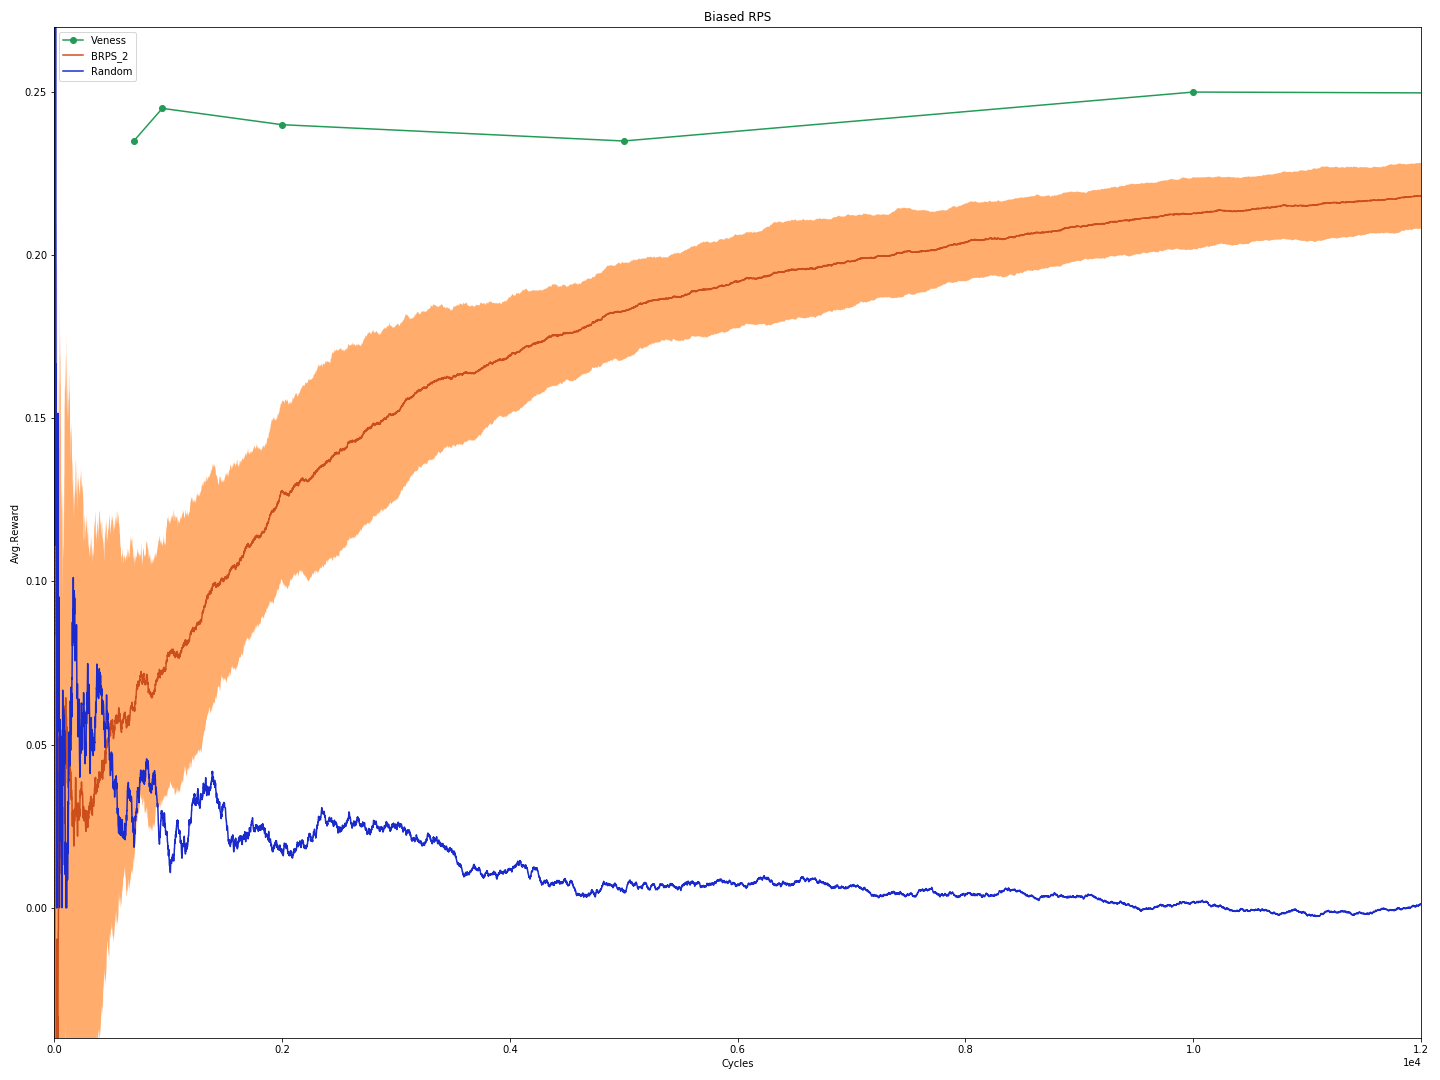
\includegraphics[width=9cm]{RvVvU_Biased_RPS}
\end{figure}

 \begin{figure}[h]
 \centering
    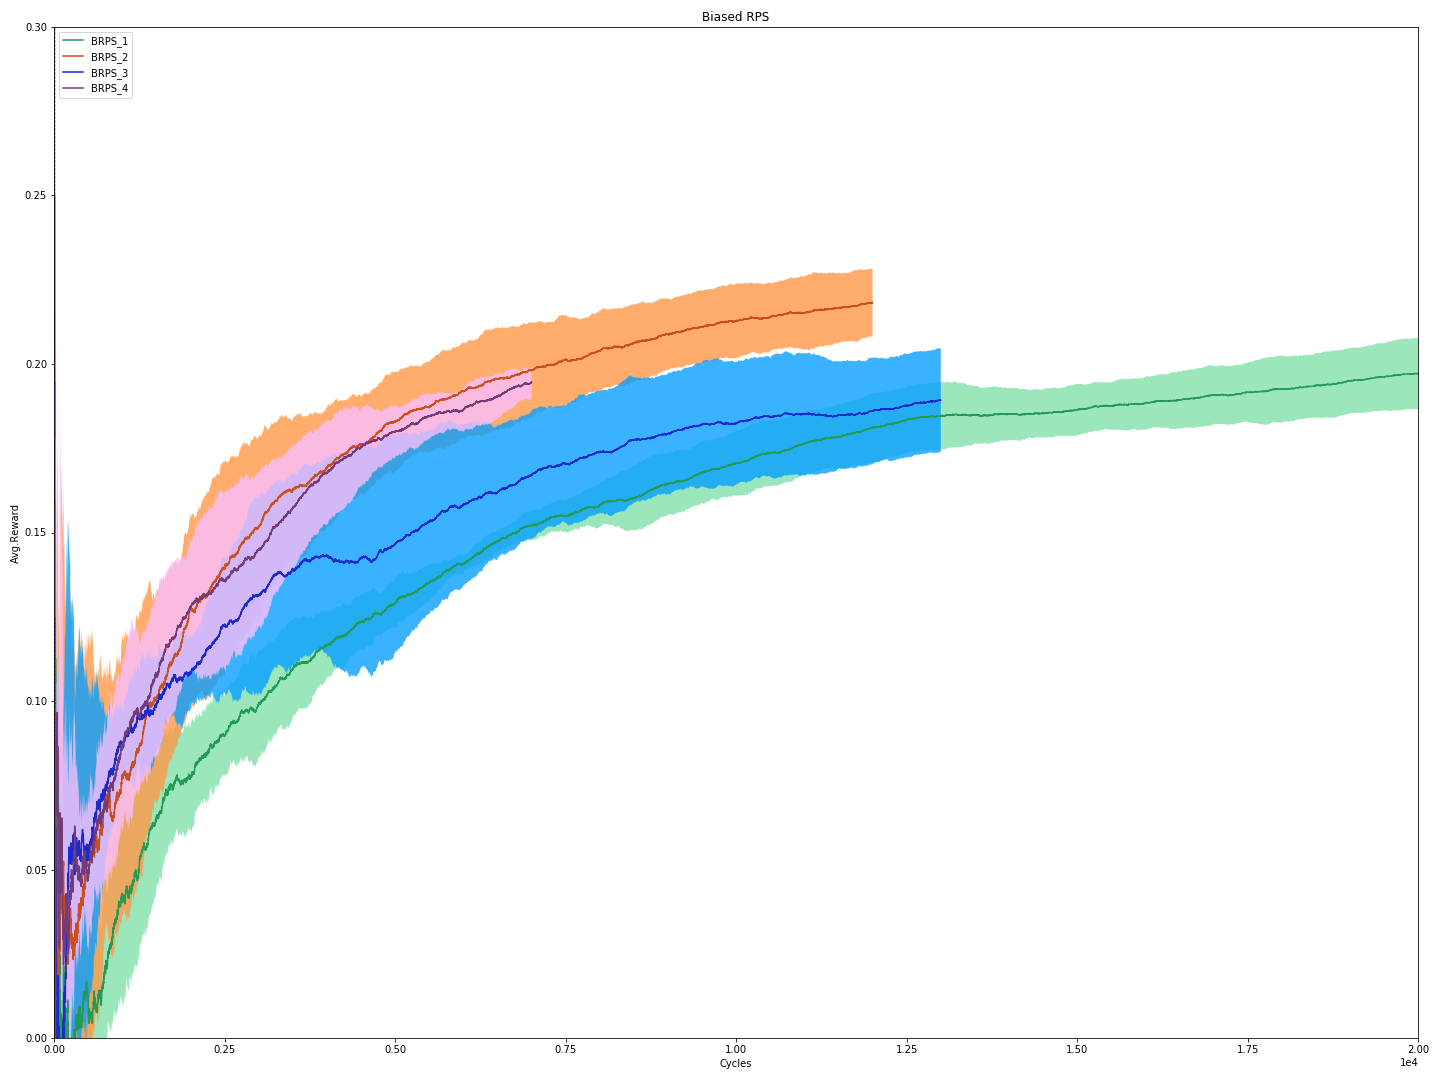
\includegraphics[width=9cm]{BT_Biased_RPS}
\end{figure}


\newpage

\subsection{Old Kuhn Poker}

\begin{tabular}{lllllll}
\centering
Environment & D & m & $\epsilon$ & $\gamma$ & Cycles & Average Reward \\
Kuhn Poker  & 42        & 2           & 0.99        & 0.9999            & 2000   & 1.2024625        \\
Kuhn Poker  & 96        & 4           & 0.9999      & 0.9995            & 24     & 1.258875         \\
Kuhn Poker  & 256       & 4           & 0.999       & 0.9991            & 13     & 1.23595         \\
%Kuhn Poker  & 512       & 8           & 0.9999      & 0.999             & 7      &               
\end{tabular}

 \begin{figure}[h]
 \centering
    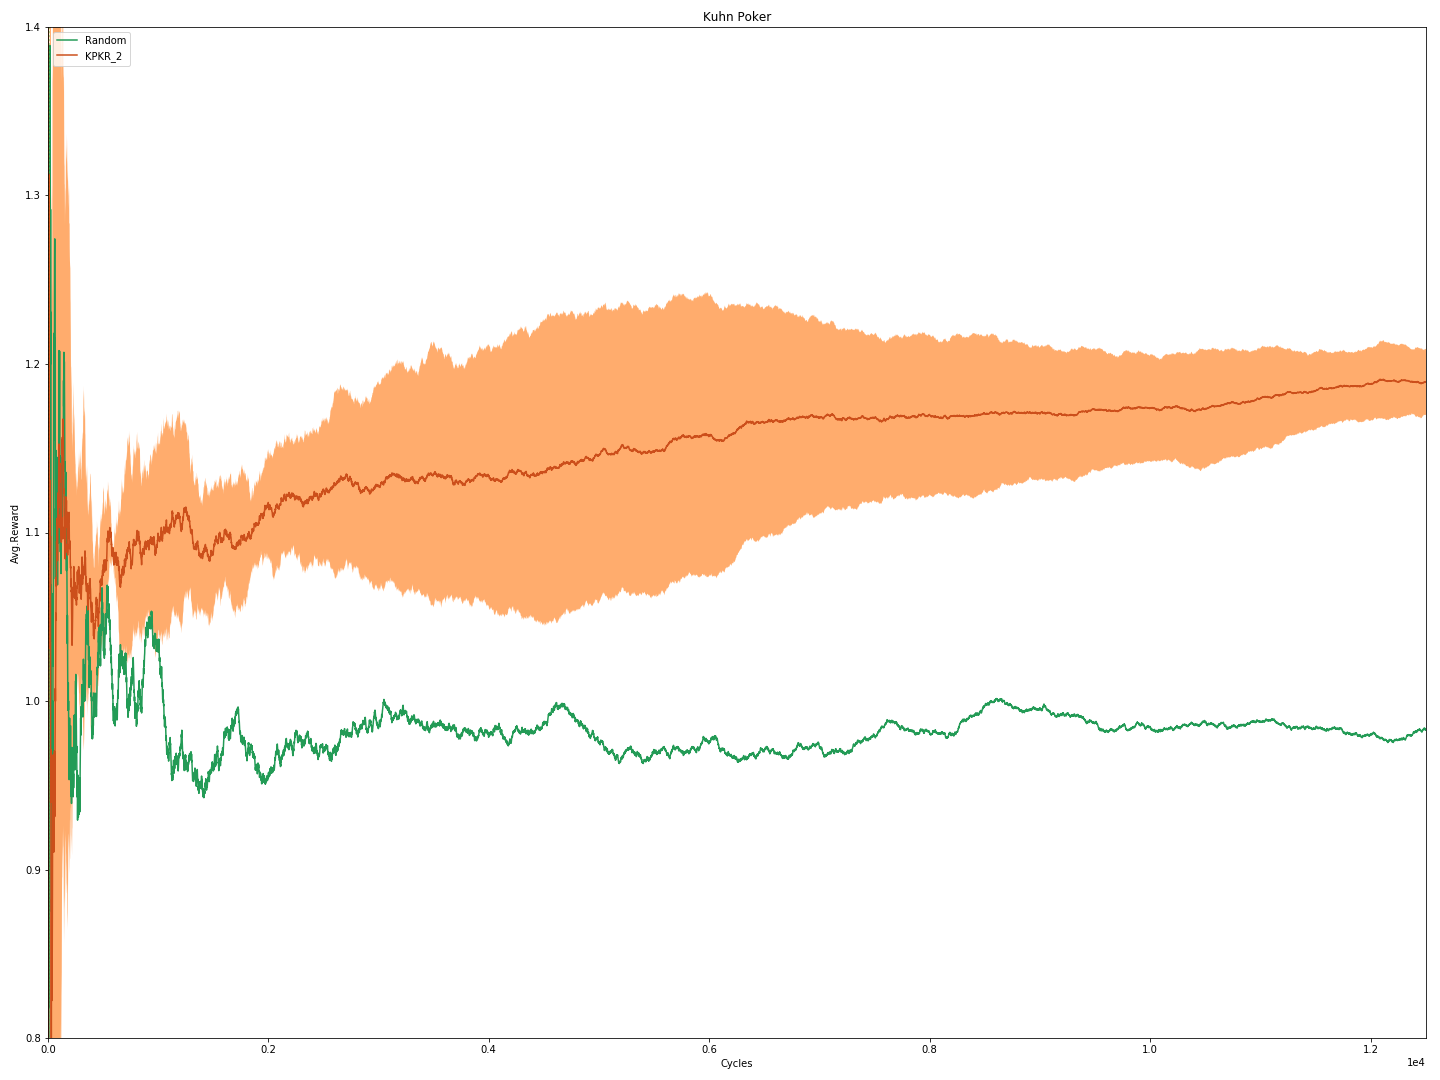
\includegraphics[width=9cm]{RvU_Kuhn_Poker}
\end{figure}

 \begin{figure}[h]
 \centering
    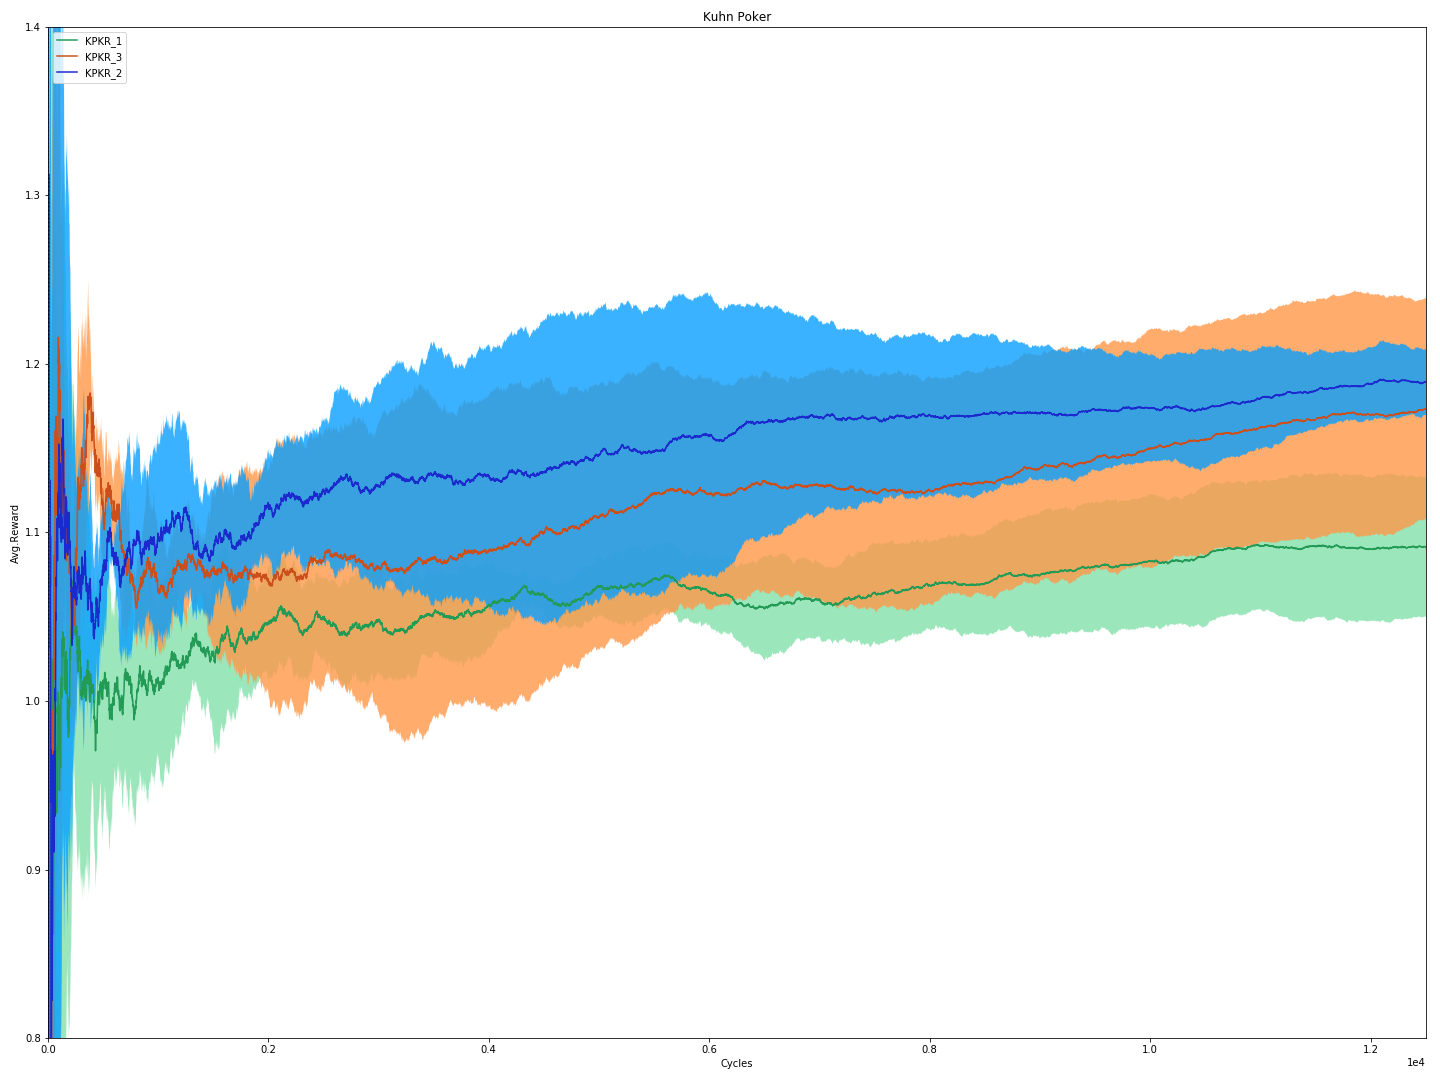
\includegraphics[width=9cm]{BT_Kuhn_Poker_2}
\end{figure}

\newpage

\subsection{True Kuhn Poker}
\begin{tabular}{lllllll}
\centering
Environment & D & m & $\epsilon$ & $\gamma$ & Cycles & Average Reward \\
Kuhn Poker  & 42        & 2           & 0.99        & 0.9999            & 2000   & 0.0719        \\
Kuhn Poker  & 96        & 4           & 0.9999      & 0.9995            & 24     & 0.01415         \\
Kuhn Poker  & 256       & 4           & 0.999       & 0.9991            & 13     & 0.0611         \\
Kuhn Poker  & 512       & 8           & 0.9999      & 0.999             & 7      & 0.056              
\end{tabular}


 \begin{figure}[h]
 \centering
    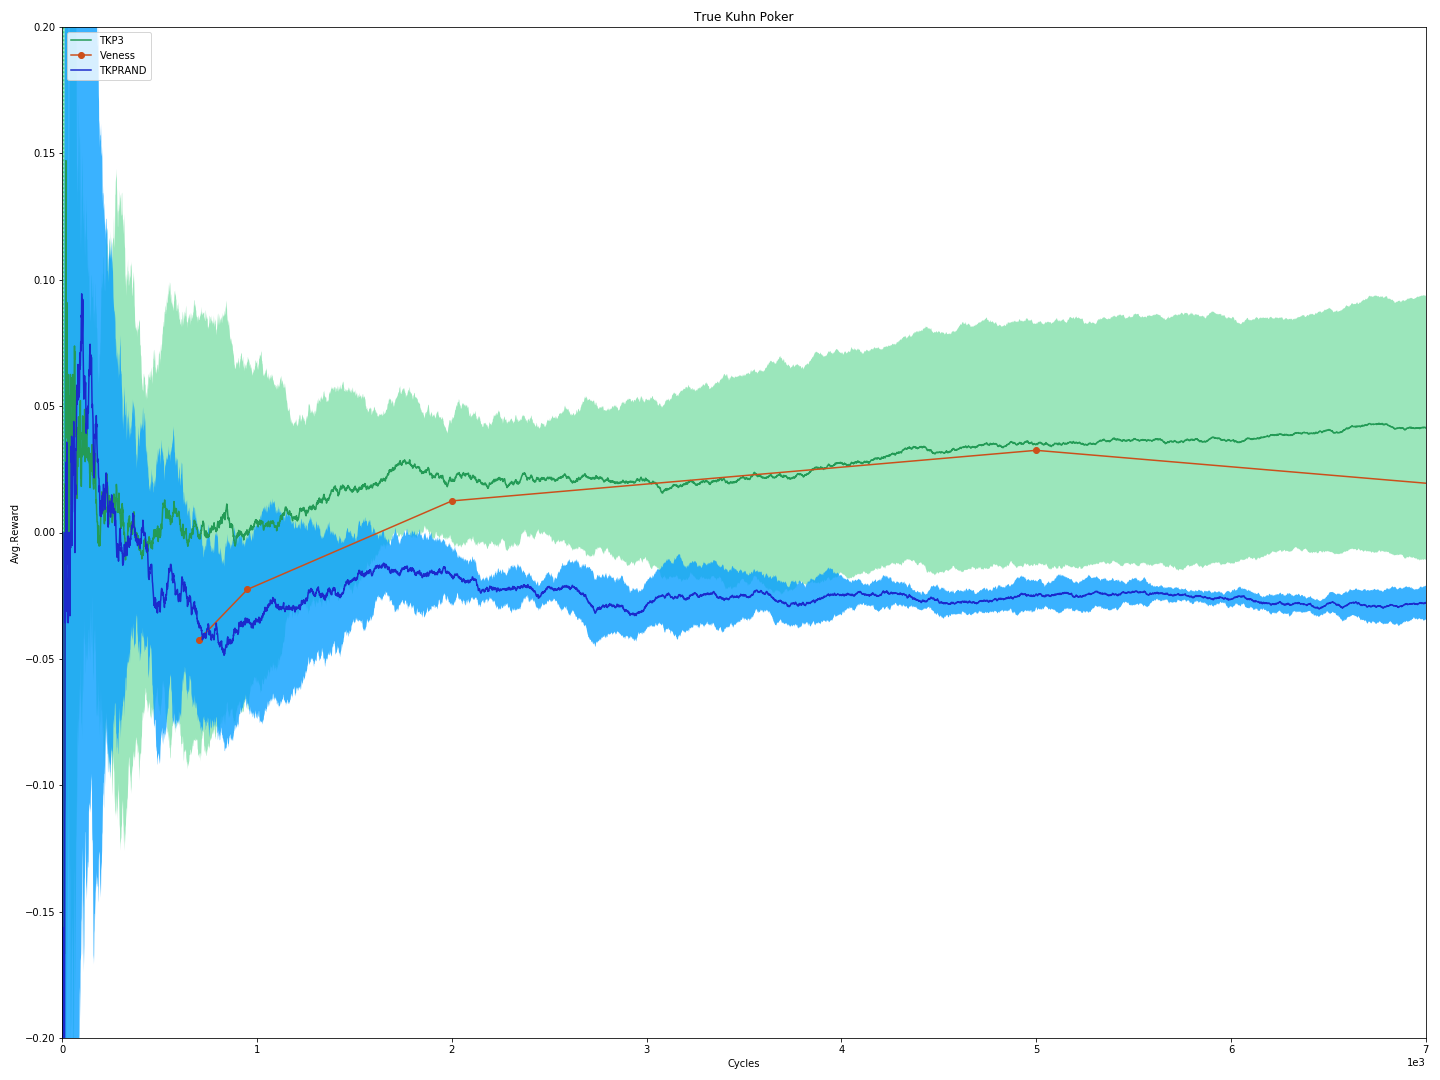
\includegraphics[width=9cm]{RvVvU_True_Kuhn_Poker}
\end{figure}

 \begin{figure}[h]
 \centering
    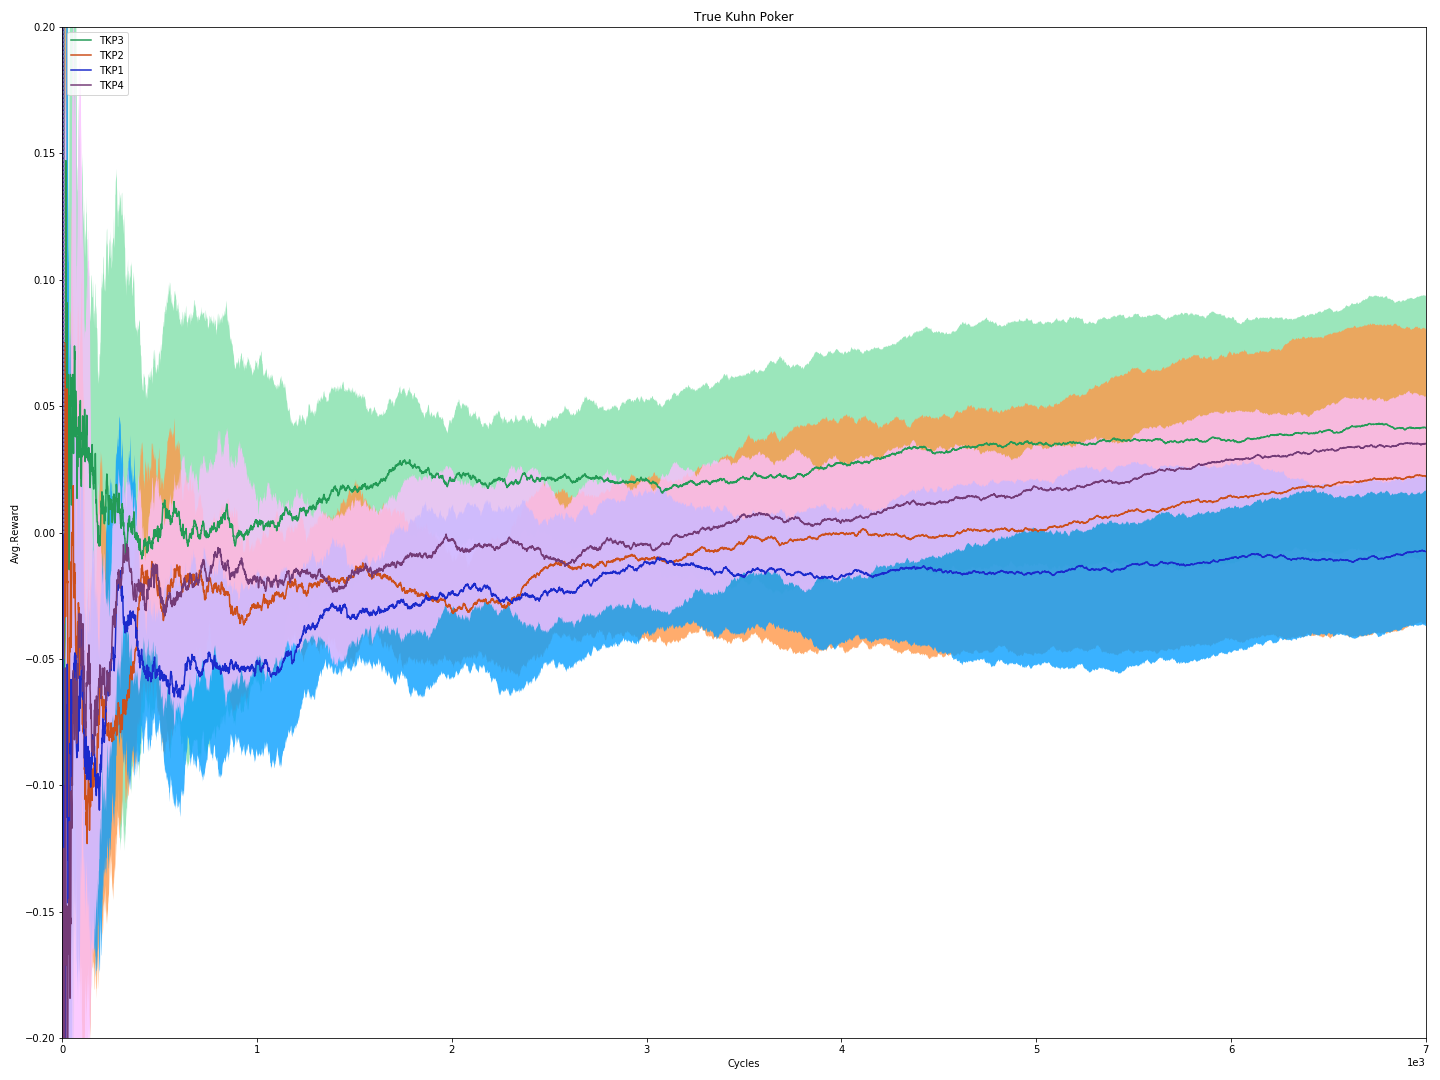
\includegraphics[width=9cm]{BT_True_Kuhn_Poker}
\end{figure}

\newpage

\subsection{TicTacToe}
\begin{tabular}{lllllll}
 \centering
Environment & D & m & $\epsilon$ & $\gamma$ & Cycles & Average Reward \\
TicTacToe   & 64        & 9           & 0.9999      & 0.99991           & 145    & 0.0661625         \\
TicTacToe   & 96        & 9           & 0.9999      & 0.9995            & 24     & -0.636375         \\
% TicTacToe   & 256       & 9           & 0.9999      & 0.9991            & 13     &                \\
TicTacToe   & 128       & 10          & 0.9999      & 0.9991            & 12     & -0.83726875        
\end{tabular}


 \begin{figure}[h]
 \centering
    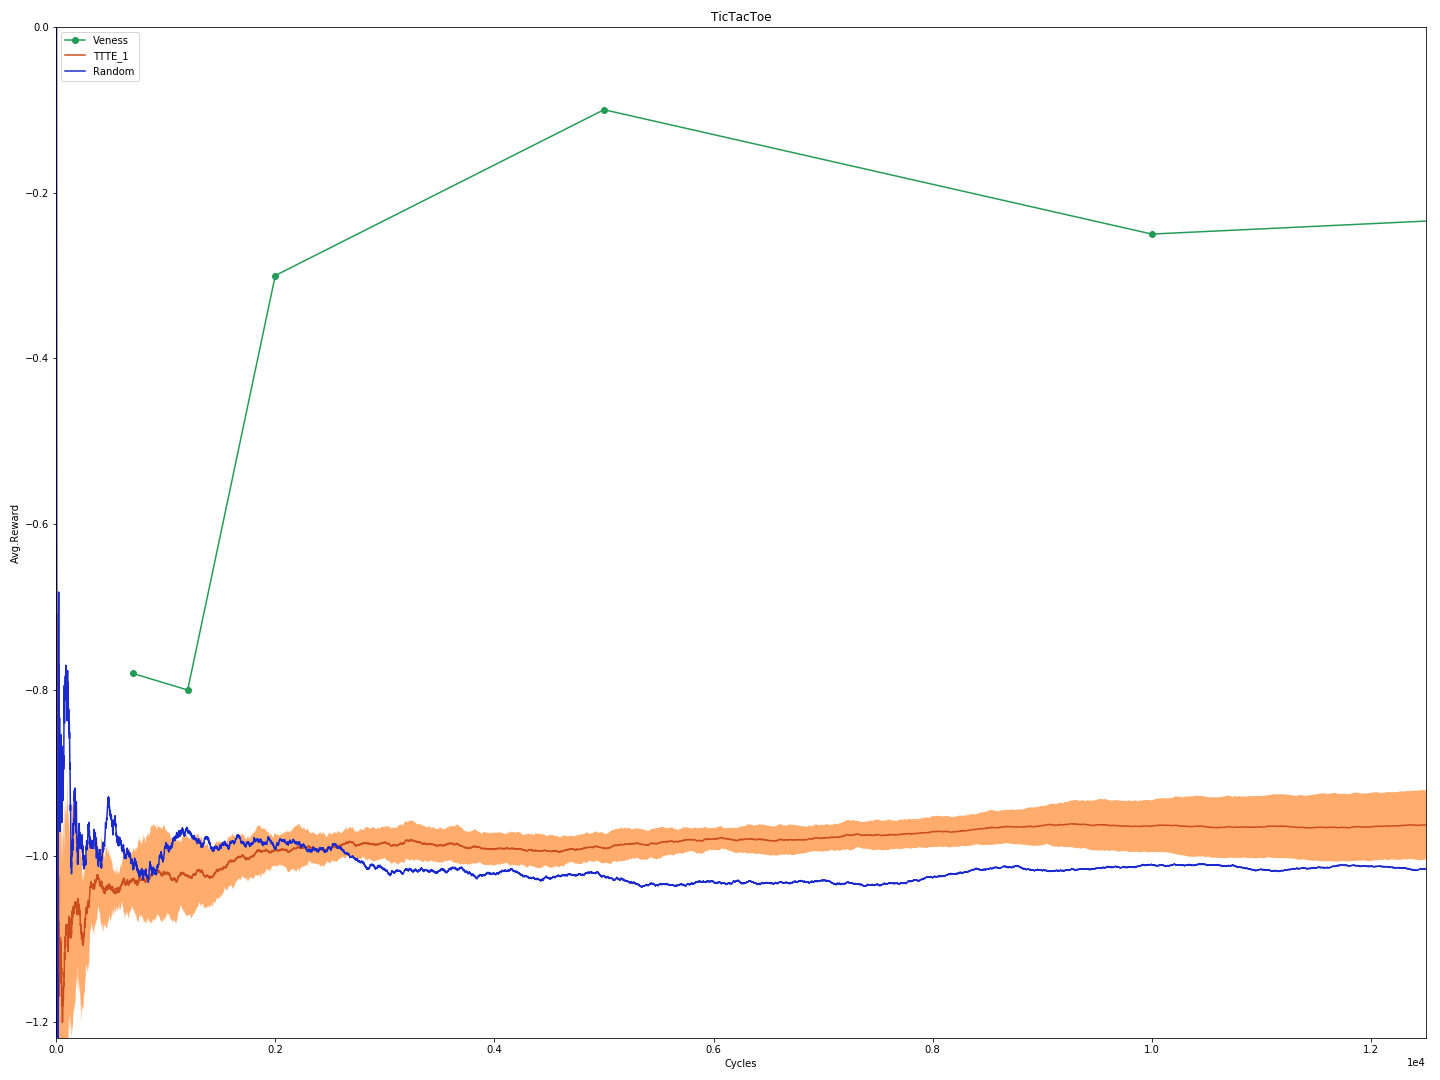
\includegraphics[width=9cm]{RvVvU_TicTacToe}
\end{figure}

 \begin{figure}[h]
 \centering
    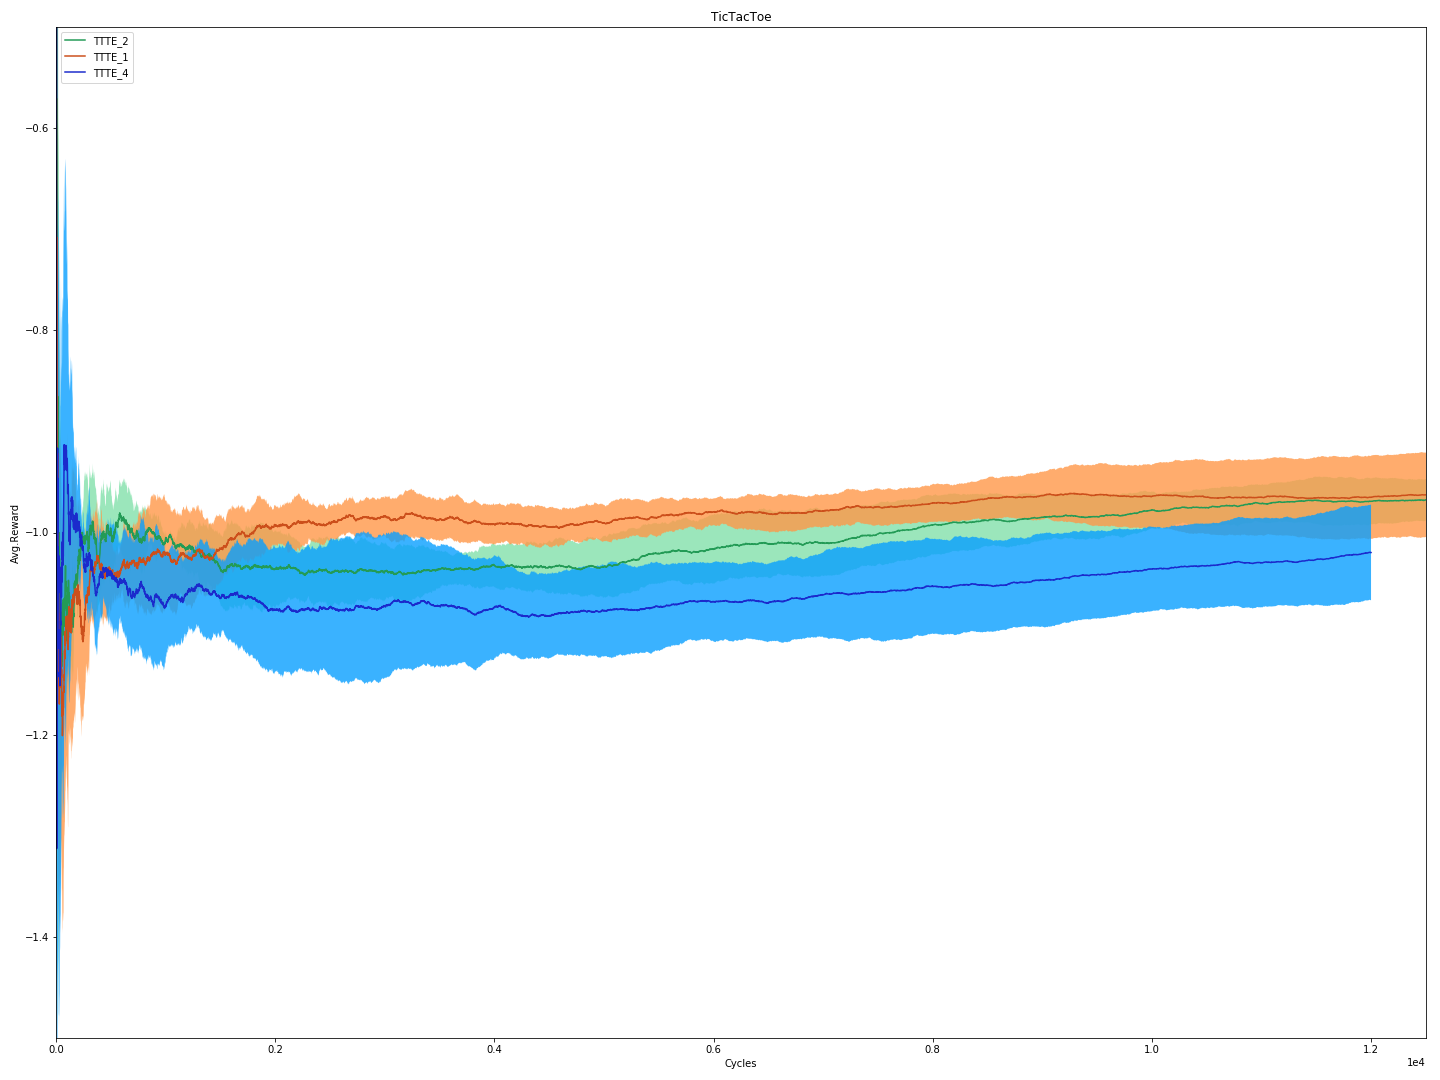
\includegraphics[width=9cm]{BT_TicTacToe}
\end{figure}


\newpage

\subsection{Extended Tiger}
 \begin{tabular}{lllllll}
  \centering
Environment    & D & m & $\epsilon$ & $\gamma$ & Cycles & Average Reward \\
Extended Tiger & 96        & 4           & 0.999       & 0.99991           & 130    & -7.77525        \\
Extended Tiger & 64        & 4           & 0.999       & 0.999             & 12     & -7.08699       \\
Extended Tiger & 42        & 8           & 0.999       & 0.9991            & 13     & -10             \\
Extended Tiger & 256       & 4           & 0.999       & 0.9991            & 13     & -7.519       
\end{tabular}

 \begin{figure}[h]
 \centering
    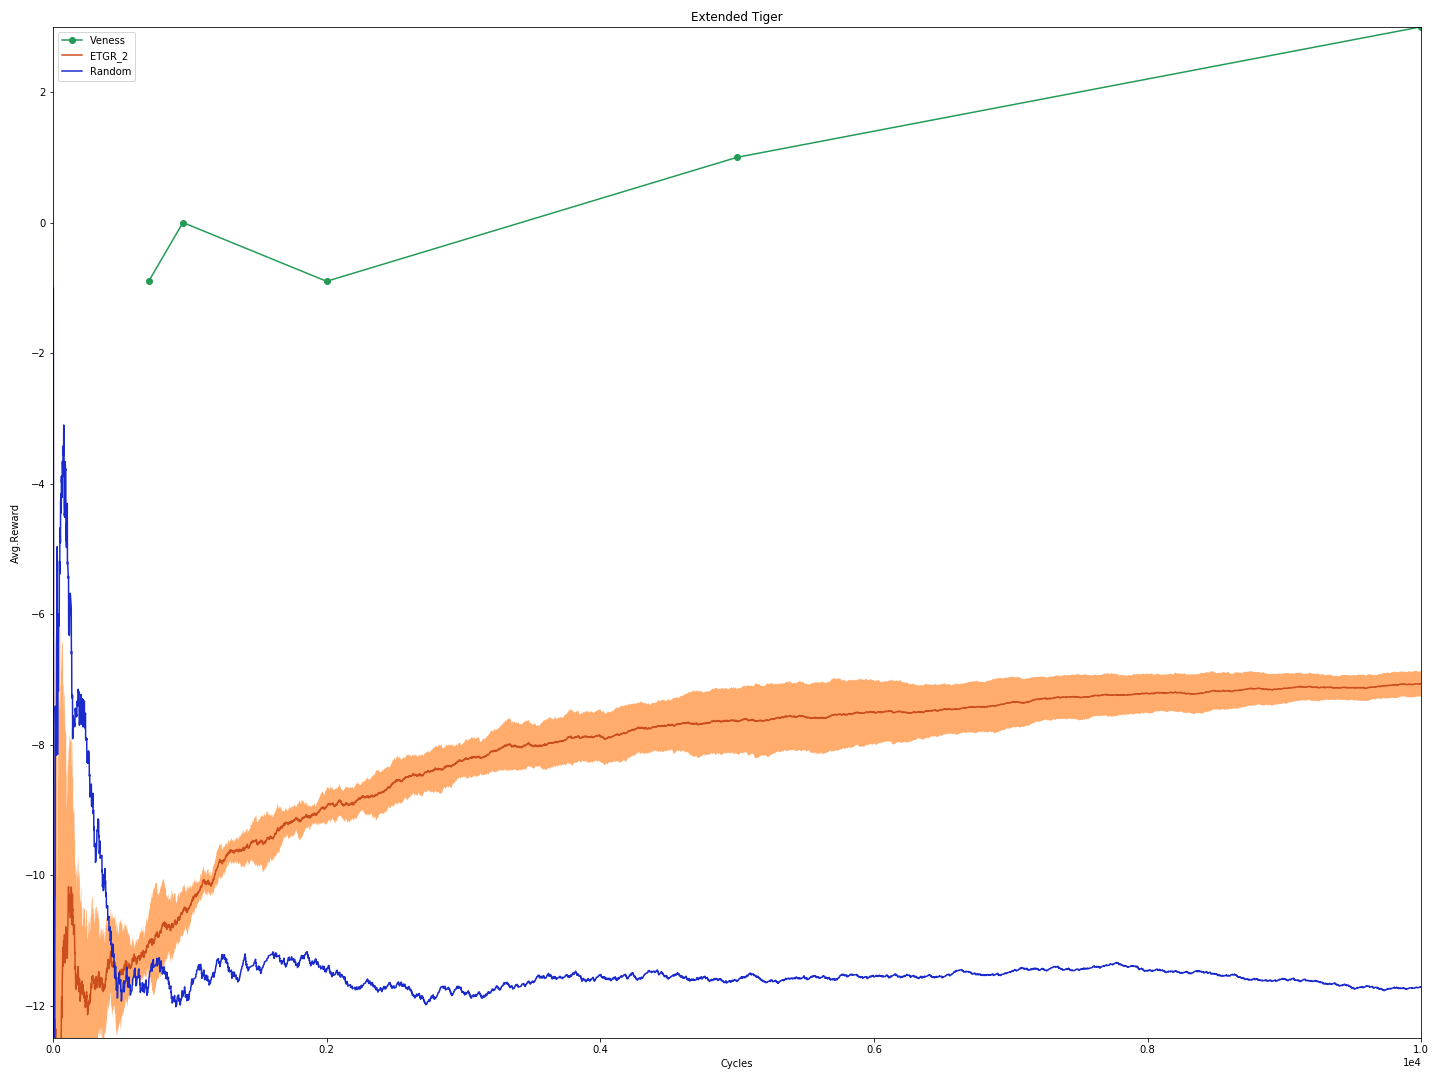
\includegraphics[width=9cm]{RvVvU_Extended_Tiger}
\end{figure}

 \begin{figure}[h]
 \centering
    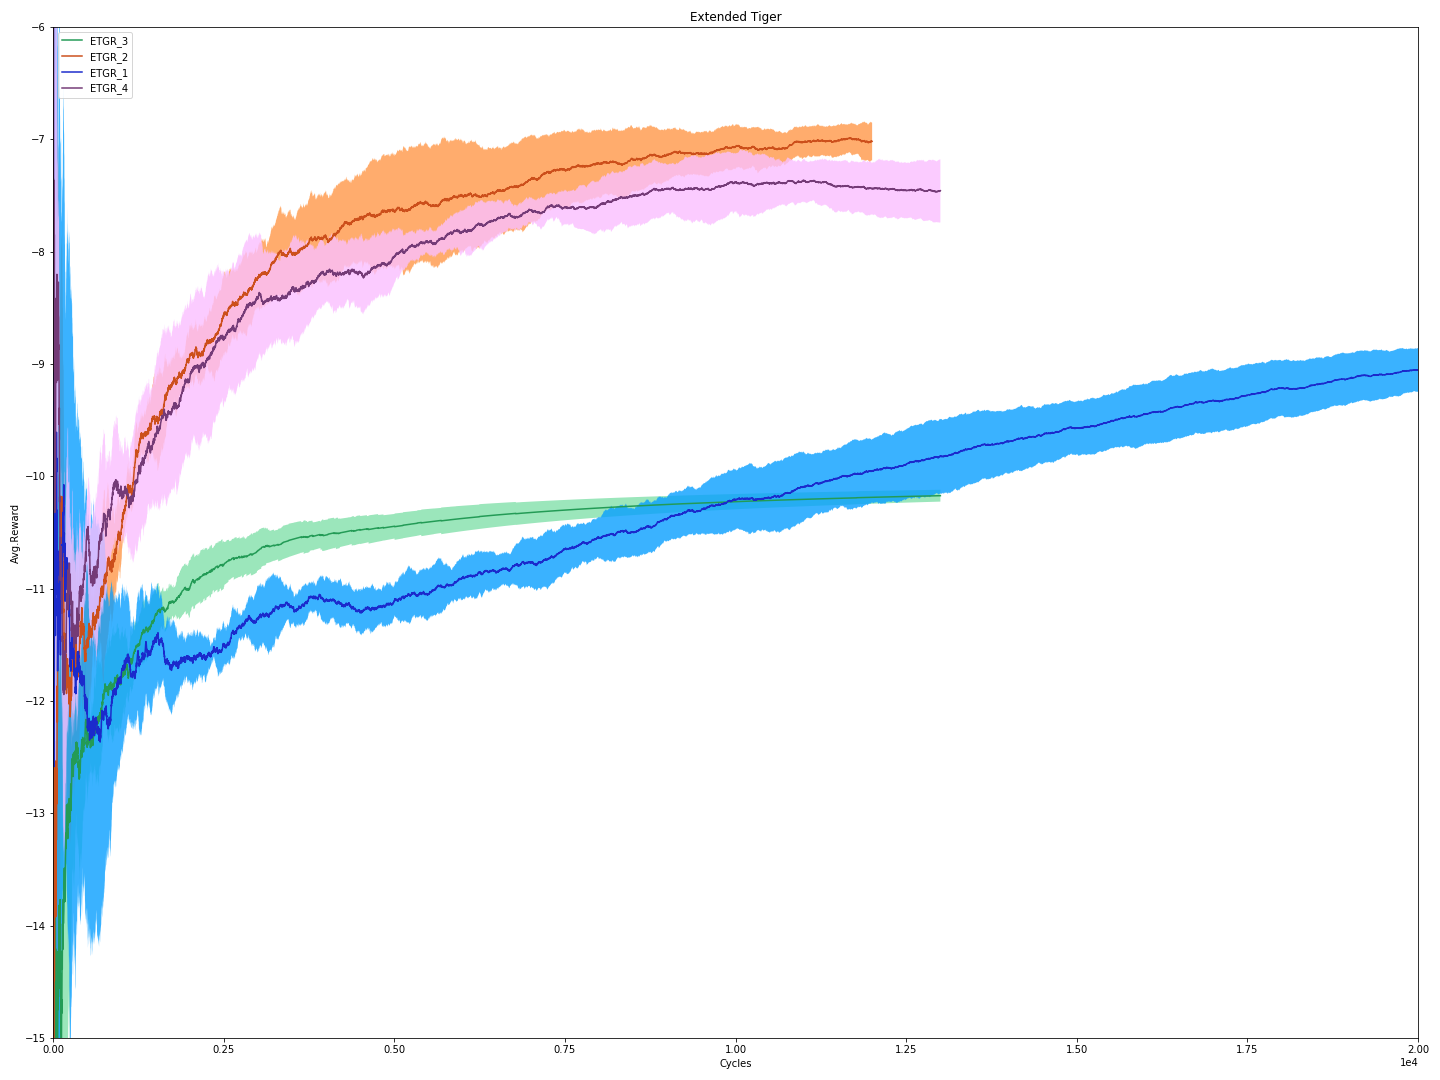
\includegraphics[width=9cm]{BT_Extended_Tiger}
\end{figure}

\newpage

\subsection{Pacman}
 \begin{tabular}{lllllll}
 \centering
Environment & D & m & $\epsilon$ & $\gamma$ & Cycles & Average Reward \\
Pacman      & 256       & 8           & 0.999       & 0.999             & 12     & -0.994        \\
%Pacman      & 512       & 10          & 0.9999      & 0.999             & 7      &                \\
Pacman      & 256       & 4           & 0.999       & 0.9991            & 13     & -1.0055625       \\
Pacman      & 92        & 4           & 0.999       & 0.999             & 7      &    -1.000225           
\end{tabular}

 \begin{figure}[h]
 \centering
    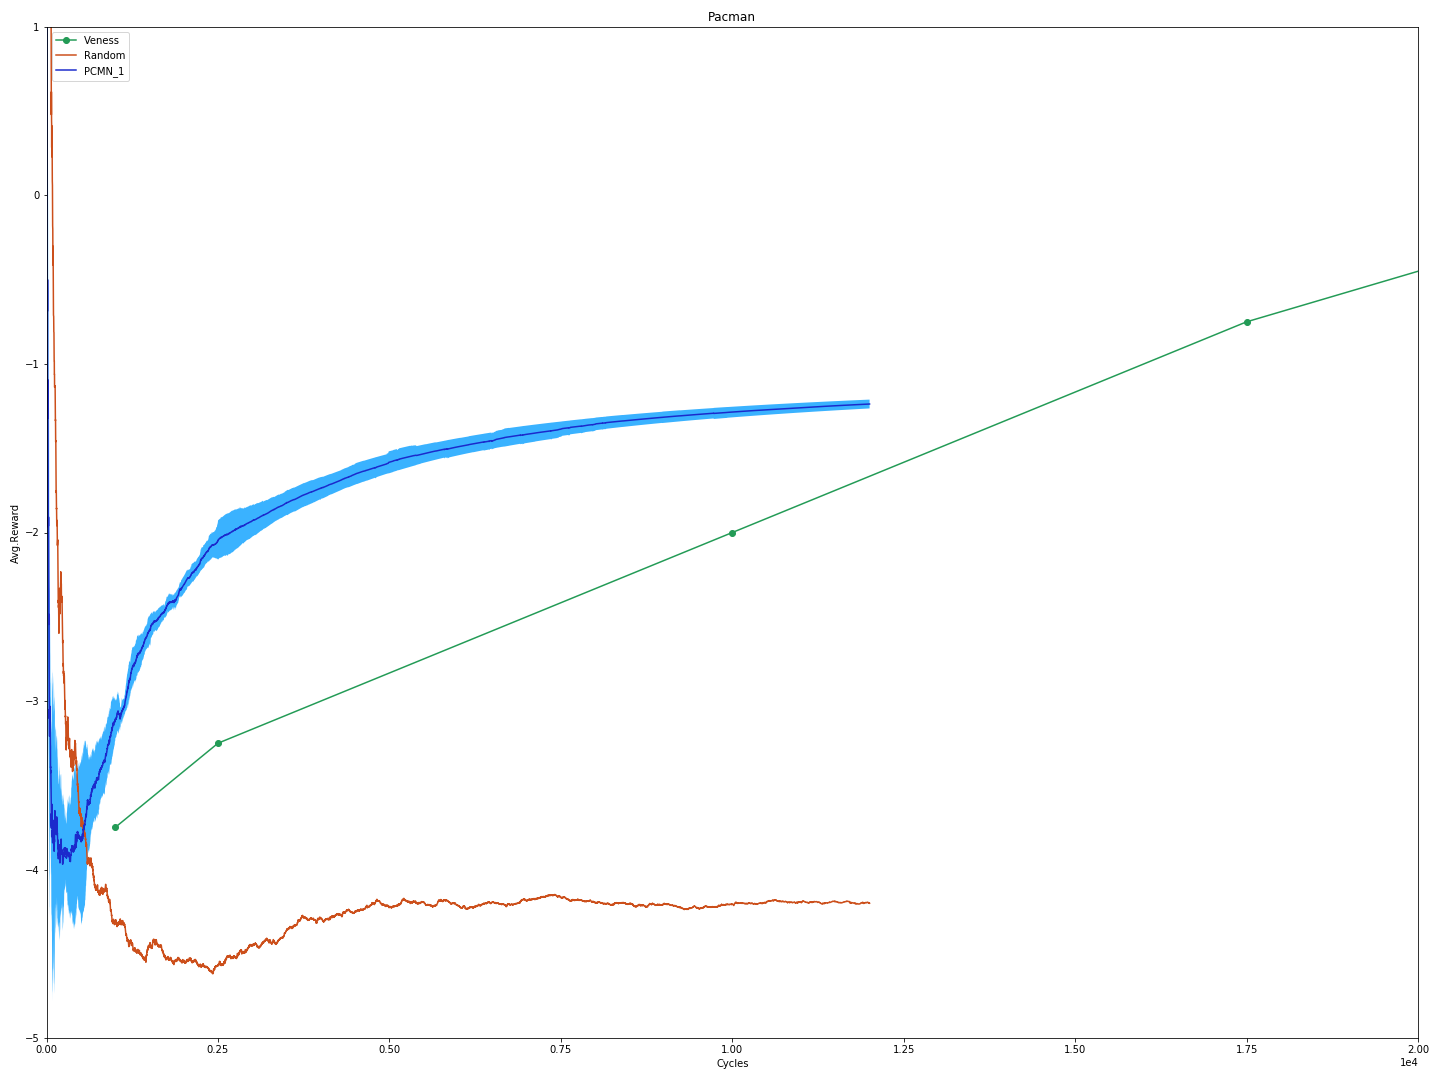
\includegraphics[width=9cm]{RvVvU_Pacman}
\end{figure}

 \begin{figure}[h]
 \centering
    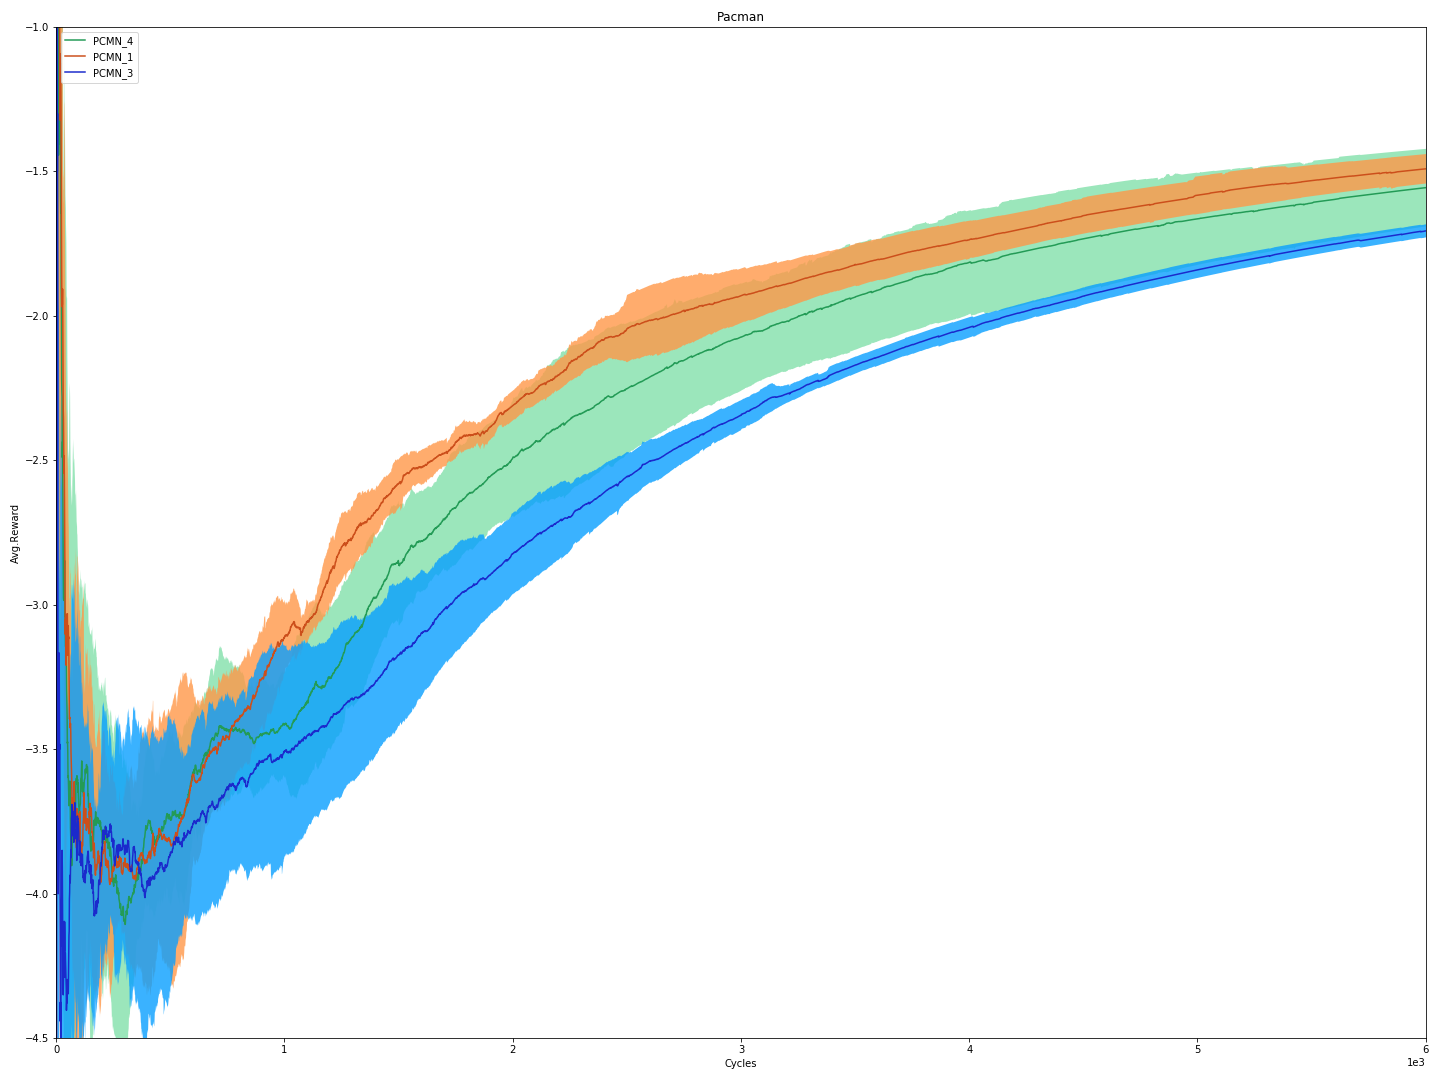
\includegraphics[width=9cm]{BT_Pacman}
\end{figure}

\newpage

\section{Discussion}


The main goal of our implementation of MC-AIXI-CTW was to achieved comparable results to \citep{veness2011monte} in the domains we chose. In this regard we were able to achieve our goal, however our graphs do not match the \citep{veness2011monte} results, this is due to our graph reflecting the average over the cycle, wheres in \citep{veness2011monte} intermediate evaluation was used. This average causes our graph to describe a $\frac{1}{x}$ graph of the reward. After training, our evaluation was comparable to \citep{veness2011monte}. Modularity was another one of the goals with our implementation of MC-AIXI-CTW. With this in mind we managed to create a loosely coupled system in which each part can be replaced easily. For example, if we wished to use Context Tree Switching \citep{veness2012context} in the place of Context Tree Weighting then the implementation required is minimal. Mentioned in \citep{veness2011monte}, the set up need not be in base 2. In fact, if base 3 was used then the observation space $|\mathcal{O}|$ of tictactoe would be reduced from $2^{18}=262144$ to $3^9 = 19683$. Another possible speedup could come from reward scaling.  e.g. for extended tiger, scaling rewards of 0,90,99,130 to 0,9,10,13. This would reduce the reward bits from 8 to 4, and be an improvement to computation time. One improvement we tested our agent on was the RoboCup simulation environment. However, in this environment our agent was unable to our perform a random agent. This was likely due to the large search space of the environment. One way in which we may we able to reduce the state space of RoboCup simulation (and possibly other environments) is through state aggregation, that is, converting equivalent or similar states to same states, thus reducing the observation (and reward) space, reducing search space, reducing computation time.


\section{Conclusion}
In all the environments we tested our MC-AIXI-CTW agent was able to outperform a random agent. Additionally, we were able to achieve comparable results to (Veness et al. 2011) for all environments. Our MC-AIXI-CTW agent can achieve near optimal to optimal solutions on small domains, however runs into difficulty for larger domains, this comes into play especially for TicTacToe, Pacman and Extended tiger.




  
  
  

\printbibliography



\end{document}
